\chapter{Über Kojo}
\begin{multicols}{2}
\section*{\color{black}Was ist Kojo?}
Kojo ist eine App die hilfen Sie programmieren zu lernen. Mit Kojo, Sie können in der modernen und leistungsfähigen Programmiersprache Scala kodieren. Kojo ist kostenlos und gibt auf Deutsch. Kojo funktioniert mit Linux, Windows und Mac OSX.
\section*{\color{black}Wo finde ich Kojo?}
Download Kojo: 
\href{http://www.kogics.net/kojo-download}{www.kogics.net/kojo-download}
Lesen Sie hier mehr: 
\href{http://lth.se/programmera}{lth.se/programmera}

\columnbreak

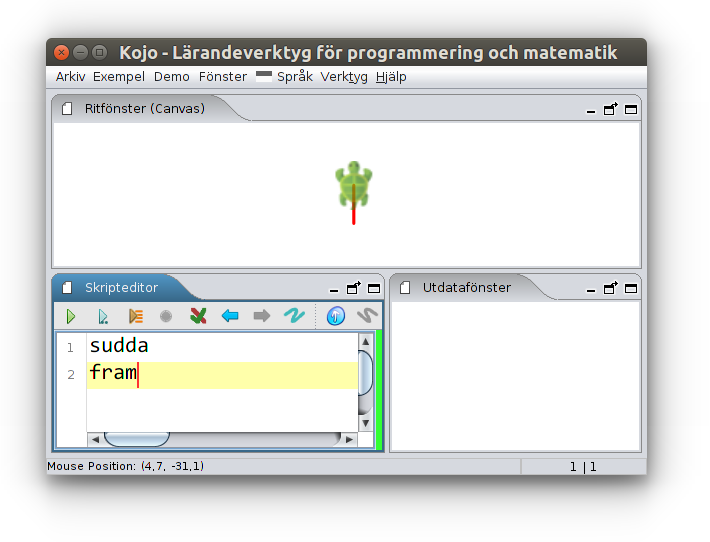
\includegraphics[width=14cm]{../img/kojo.png}
\end{multicols}

\chapter{Ihr erstes Programm}
\begin{multicols}{2}
\section*{\color{MidnightBlue}Sie lernen:}
Schreiben in einem Editor.\\
Ein Programm starten.
\section*{\color{BrickRed}Aufgabe:}
Schreiben Sie das Programm im Editor:

\begin{lstlisting}[basicstyle={\ttfamily\fontsize{24}{24}\selectfont}]
clear
forward
\end{lstlisting}
        
Drücken Sie die grüne Play-Taste \\
 um kick off Programm.

\columnbreak

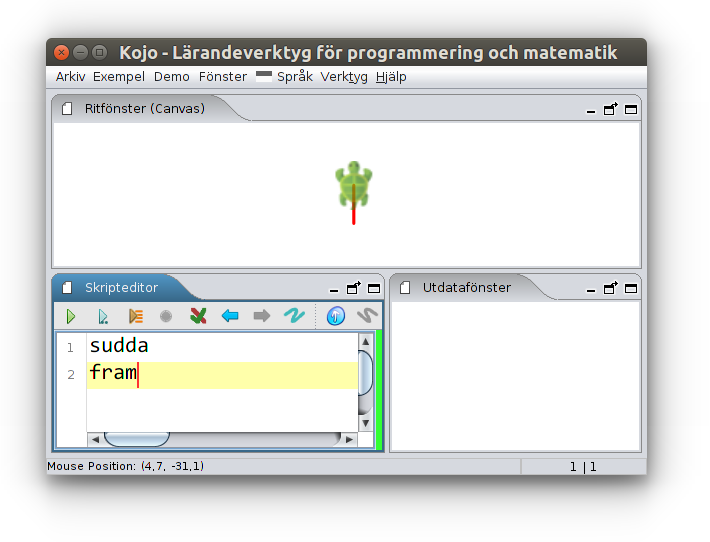
\includegraphics[width=14cm]{../img/fram.png}
\end{multicols}

